\documentclass{./styles/svproc}

\usepackage{url}
\usepackage{biblatex}
\usepackage{graphicx}
\usepackage{amsmath,amssymb,amsfonts}%

\bibliography{./styles/bibtex/sn-bibliography}

\def\UrlFont{\rmfamily}
\begin{document}
\mainmatter 

\title{Unmask Masked Face}
\titlerunning{Unmask Masked Face}

\author{Harshit Timmanagoudar{*} \and Preethi P}
\authorrunning{Harshit Timmanagoudar et al}
\institute{Department of Computer Science, PES University, Bangalore, 560085, Karnataka, India,\\
\email{harshit.utd@gmail.com},
\email{preethip@pes.edu}}

\maketitle 

\begin{abstract}
Deep neural network-based realistic image synthesis has gain-ed popularity as a research topic in the fields of machine learning and computer vision. The ability to generate unmasked photographs of people from their masked counterparts is a fascinating research topic with potential applications in numerous fields. In order to solve the issue of mask-to-unmask picture synthesis, conditional generative adversarial networks (cGAN) are used in this article. We introduce the Pix2Pix model, which can handle both the overall structure of the entire image and the fine details of a particular area, for creating unmasked images from masked ones. Later in the investigation, using subjective analysis, we discover that the Pix2Pix model effectively creates realistic unmasked photos.
\keywords{GAN, cGAN, Pix2Pix, Generator model, Discriminator mo-del}
\end{abstract}

\section{Introduction}
The purpose of this research article is to investigate if it is possible to automatically remove substantial items from facial photographs, such as face masks. This study focuses on the unmasking of masked faces since it is a fascinating subject with significant practical implications. Mask use has increased because of a variety of factors, such as worries about COVID-19, pollution, or an illness. Wearing masks, however, also prompts worries about disguised people engaging in unlawful activity, making it hard to pin-point the culprits. Hence, removing the mask or any other item that covers a sizable section of the face may help identify the individual. To generate a complete facial image of an individual, it can be challenging task to match the facial components that are partially seen, like the shape of the nose, skin complexion, and facial hair (if present).

To tackle this challenge, early methods that were not based on machine learning \cite{1323101}, \cite{Darabi2012} would remove the obscuring objects and generate replacement content identifying similar patches from other parts of the image. Another approach, outlined in \cite{Hays:2007}, involved locating comparable patterns from a vest database of scene images and placing them into the damaged region. Although these methods are successful in removing the objects, they are restricted to removing only small objects from images and do not produce desirable and realistic images.

Numerous machine learning-based techniques have emerged to improve image editing algorithms, surpassing non-learning methods for the removal of unwanted objects from images. A noteworthy instance is presented in \cite{article0}, where researchers have developed an innovative approach based on Generative Adversarial Networks (GANs) to eliminate masked objects. Their method comprised two steps: creating a binary segmentation of the masked picture in step one, and then removing the masked area and producing the affected region using a generator model and two discriminator models in step two. In contrast, our research aims to accomplish unmasked areas without requiring binary segmentation of the masked region, and by employing a single discriminator model. In other words, our approach strives to directly eliminate the masked objects from the image and generate the missing areas, avoiding the intermediate step of generating a binary segmentation.

\section{Related Work}
In the Generative Adversarial Networks (GAN) \cite{goodfellow2014generative} paradigm, an adversarial contest is employed to train a generator model and the discriminator model.The discriminator builds the ability to differentiate between the actual data samples and artificially synthesised ones. In order to con the discriminator into categorising synthesised samples as genuine, the generator has been specifically developed to do just that. This neural network called the generative adversarial network, or GAN, for short, is formed to learn a mapping between random noise and the output image. $i \rightarrow k$,  where $i$ refers to random noise and $k$ refers to the output image. The generator, indicated as $G$, is in charge of creating fake pictures that appear as though they may have been created using the same distribution as the actual photos. A discriminator network, indicated as $D$, that has been trained to discern actual pictures from counterfeits ones, assesses the effectiveness of the generator. While the generator tries to produce images that can't be distinguished from the genuine ones, the discriminator tries to properly determine if the images are real or fake. The usage of GANs for image synthesis jobs has increased. The many GAN varieties are summarised in the article \cite{8195348} along with how they may be used to applications like super-resolution, style transfer, and image-to-image translation.

Conditional GANs (cGAN), on the other hand, are conditioned to certain information to the learn the mapping between the corresponding images \cite{mirza2014conditional} i.e. to learn a mapping $j \rightarrow k$, where $j$ refers to the observed image and $k$ as mentioned before refers to the output image. The Pix2Pix GAN is a conditional GAN, which implies that the yield of the output image is conditioned on an input image, in contrast to conventional GANs that produce random images from a noise vector. These networks have employed in various research works such as cartoon image generation \cite{liu2017autopainter}, shadow synthesis of virtual objects \cite{Zhang2019}, prognosis prediction for breast cancer \cite{Zhang2022}, determination of optimal path route in autonomous robot systems \cite{9366777} and many more applications. 

In Image-to-Image \cite{isola2018imagetoimage}, the authors put forward a method named "Pix2Pix" that employs a "U-net" design \cite{ronneberger2015unet} to address the task of image-to-image transfer in a broad sense. This approach enables the decoder to utilize information from encoder layers for better conditioning. Pix2Pix GAN has been employed for various purposes such as data augmentation \cite{Toda2022} \cite{Hlscher2022}, colorization and classification of intracranial tumor expanse in MRI images \cite{Mehmood2022} and many image-to-image translation tasks such as image of daylight to night, and city images from map.

\section{Methodology}
In both the GANs and cGANs scenarios, the generator and discriminator networks are trained concurrently using a minimax game. While the discriminator aims to maximise classification error, the generator strives to minimise it. The generator is urged to produce images that resemble real ones more and more, making it harder and harder for the discriminator to distinguish between them. The discriminator model is updated directly by comparing its classification result to the ground truth label, but the generator model is updated via the discriminator model during training. This is accomplished through an adversarial process in which the discriminator model seeks to more effectively identify phoney images while the generator model seeks to more effectively deceive the discriminator by creating more convincing images. The training process of typical Pix2Pix GAN can be visualized with help of the Fig 1.

\begin{figure}[ht]%
\centering
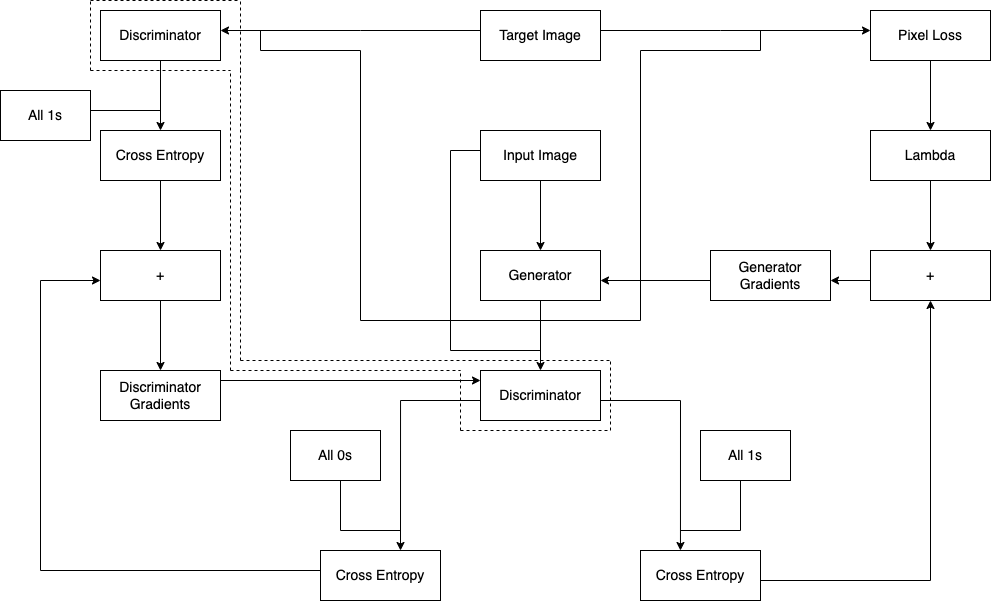
\includegraphics[width=0.95\textwidth]{figures/training.png}
\caption{Training Process Flow of Pix2Pix GAN for synthesizing unmasked realistic images from the corresponding masked images.}\label{fig1}
\end{figure}

In Fig 1, the two discriminator blocks refer to the same discriminator model. For each input masked picture, the generator creates an output image throughout the training phase. The first inputs to the discriminator are the generated unmasked picture and the input masked image. The real unmasked picture and the input masked image make up the second input. By doing this, the discriminator is able to distinguish between how the input picture is translated into the actual and synthesised outputs. The generator loss is a mix of adversarial loss impacted by the discriminator and the task-specific loss function, such the L1 loss, in a certain ratio, and the generator loss is calculated as the next phase in the training process. By adding more variety and vividness to the generated images, the adversarial loss aids in the creation of more realistic visuals. The L1 loss describes the pixel-level difference between the produced picture and the original image. The gradients of the loss are then computed and applied to the optimizers with regard to the generator variables and the discriminator variables. In this approach, the training process helps the discriminator recognise a picture as real or false and the generator produce more realistic images.

\subsection{Generator}

The main function of the generator in a Pix2Pix GAN is to take an input image and create an output image that has been transformed or translated based on a particular task or objective. Unlike traditional GANs, which randomly generate images from a noise vector, the Pix2Pix GAN is a conditional GAN that trains both the generator and the discriminator on paired input and output images.

A Pix2Pix GAN typically has an encoder-decoder architecture for the generator that incorporates skip connections between the encoder and decoder layers to preserve spatial information. The encoder component of the generator creates feature maps of various sizes by continuously downsampling the input image while also capturing the essential information needed to synthesise or generate a new image in the future. The feature map obtained from the architecture's bottleneck is continually upsampled in the decoder portion of the generator to produce a new image with the same size as the input image. The feature maps are also upsampled by the decoder layers utilising the information recorded at the relevant encoder layer thanks to the skip connections. The generator can maintain fine-grained details while generating high-level features because to the skip connections in the U-Net design. The usage of a U-Net architecture by the generator in a Pix2Pix GAN is one of its distinctive characteristics. A symmetrical structure with a contracting path in the encoder and an expanding path in the decoder distinguishes this architecture. The generator can maintain fine-grained details while generating high-level features because to the skip connections in the U-Net design.

The generator model is trained using adversarial loss with the backing of the discriminator and task-specific loss function, such as L1 loss. The generator model's goal is to transform input images from one realm to another, or to convert masked images of people to unmasked images of those people in our case. In order to achieve the objective or the goal, the generator and the discriminator model are put up to challenge each other. The generator intends to synthesise images that delude the discriminator into segregating them as real, while the discriminator's goal is to segregate the real target images and the generator's synthesised images.

The L1 loss incorporated in addition to the adversarial loss quantifies the pixel-wise difference between the ground truth images and the corresponding synthesised images. In a bid to encourage the generator to create output images that closely resemble the desired target domain, the L1 loss must be kept to a minimum. Strong supervision from the L1 loss ensures that the generator picks up the target images' structural and perceptual specifics.

The adversarial loss and the L1 loss are combined in a weighted manner during training to determine the generator's total loss. Gradient-based optimisation techniques are used to reduce this total loss. By combining the two losses, the generator is trained to produce realistic and eye-catching images that not only trick the discriminator but also display faithfulness to the intended domain. The Pix2Pix GAN framework produces high-quality, visually cohesive images as a result of the interaction between the adversarial loss and the L1 loss.

The architectural design of the generator model can be visualized with help of Fig 2.

\subsection{Skip Connections}

The Pix2Pix GAN (Generative Adversarial Network) design relies heavily on skip connections, sometimes referred to as residual connections. They serve to improve communication between the network's input and output, which ultimately raises the calibre of image translation. These connections enable the network to learn high-level representations through deeper layers while also allowing the generator to retain low-level features from the input image.

Skip connections are created by directly coupling the early layers of the encoder with the layers of the decoder that correspond to those early levels. The input image undergoes a sequence of convolutional layers during the encoding stage that gradually shrink its spatial dimensions and capture abstract representations. The encoder's outputs are recorded for subsequent use at each phase of the downsampling process.

To create the output image during the decoding phase, the decoder uses the encoded characteristics and gradually upsamples them. The stored encoder outputs (skip connections) are element-wise concatenated or summed with the upsampled features at each upsampling step. Through this approach, the decoder may access both the high-level representations that the encoder has learnt and the low-level features from the input image. Skip connections enable the generator to create crisper and more aesthetically pleasing output pictures while preserving fine-grained details and overall structure.

As a result of facilitating the merging of low-level and high-level characteristics, skip connections are crucial in Pix2Pix GANs. They let information move more easily between early and later layers, which enhances the quality of picture translation. Skip connections help the generator produce aesthetically appealing and correct output pictures by keeping track of crucial features and letting the network acquire abstract representations.

\begin{figure}[ht]%
\centering
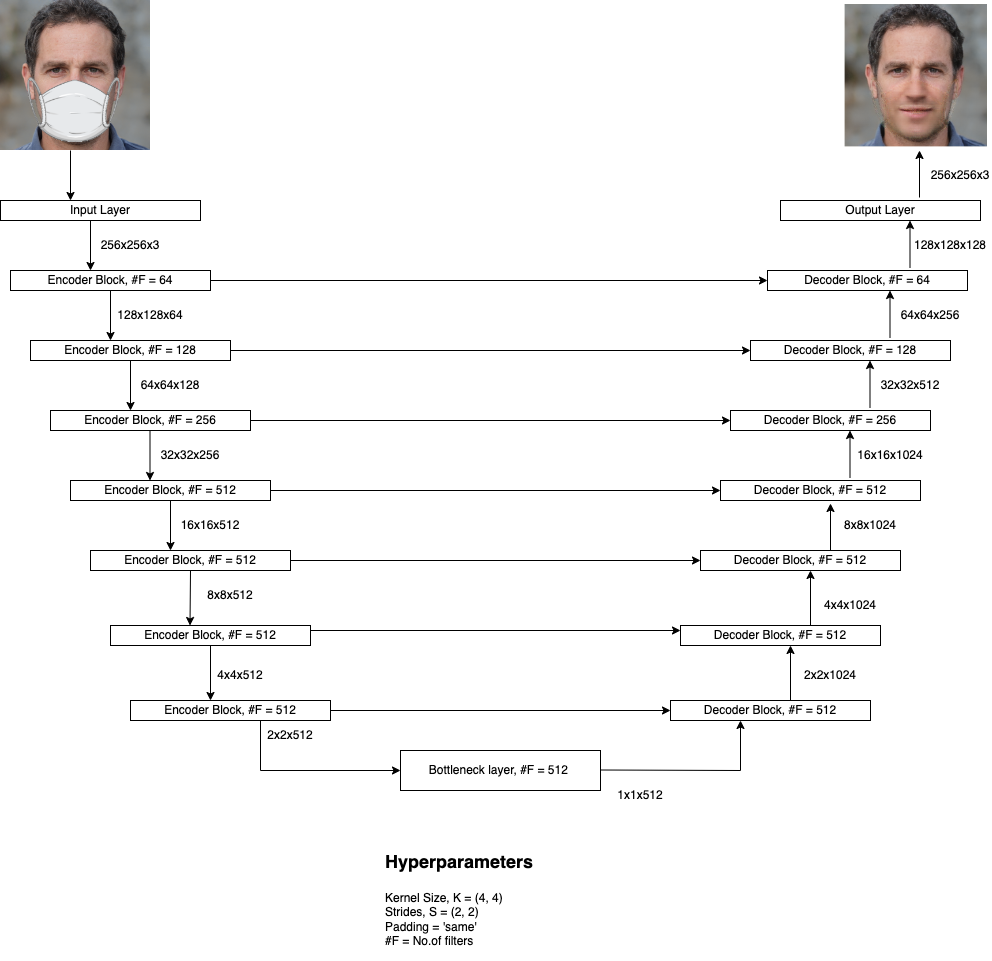
\includegraphics[width=0.95\textwidth]{figures/generator.png}
\caption{Architectural Design of the Generator Model. The encoder, which down samples the input picture while collecting key characteristics, is located on the left side of the design. The decoder, which up samples the features and attempts to rebuild the picture using the data received from the skip connections, is the proper component of the architecture.}\label{fig2}
\end{figure}

\subsection{Discriminator}\label{subsec4}

According to the method used, conditional-image classification, which tries to categorise pictures based on their validity as a translation of the original image, was performed using deep convolution neural networks as the discriminator. This was accomplished by feeding the discriminator input for both the source and target images, which forecasted the probability that the target picture is an accurate translation of the source image.

The discriminator model in the Pix2Pix GAN plays a vital role in concluding how realistic the synthesised images of the generator model are. The discriminator model makes use of the PatchGAN architecture that lets if effectively analyse the images and gather contextual data. The input images are broken down into smaller patches by this architecture and later each patch is assessed to conclude if it real or synthesised. Rather than concentrating on the entire image, the discriminator may collect fine-grained features and make more targeted conclusions by concentrating on particular image areas.

The intent of the PatchGAN discriminator is to mitigate the effective receptive field, which refers to the area or the patch of the input image that has a consequence on the of a particular unit. The discriminator may analyse smaller regions and give the generator more comprehensive input by taking into account patches rather than the complete image. This method offers a variety of advantages. When compared to analysing the complete image, it first decreases computing complexity. Additionally, it enables the discriminator to more accurately evaluate local picture structures and textures, guaranteeing that the resulting images preserve high-quality details. Additionally, by looking at patches, the PatchGAN discriminator directs the generator to create output images that match the local image statistics of the target domain, producing aesthetically consistent results.

In a nutshell the Pix2Pix GAN's discriminator model relies on a patch-based methodology to assess the realism of produced pictures. It may collect minute details and provide the generator more accurate input by concentrating on smaller areas.

The architectural design of the discriminator model can be visualized with help of Fig 3.

\begin{figure}[ht]%
\centering
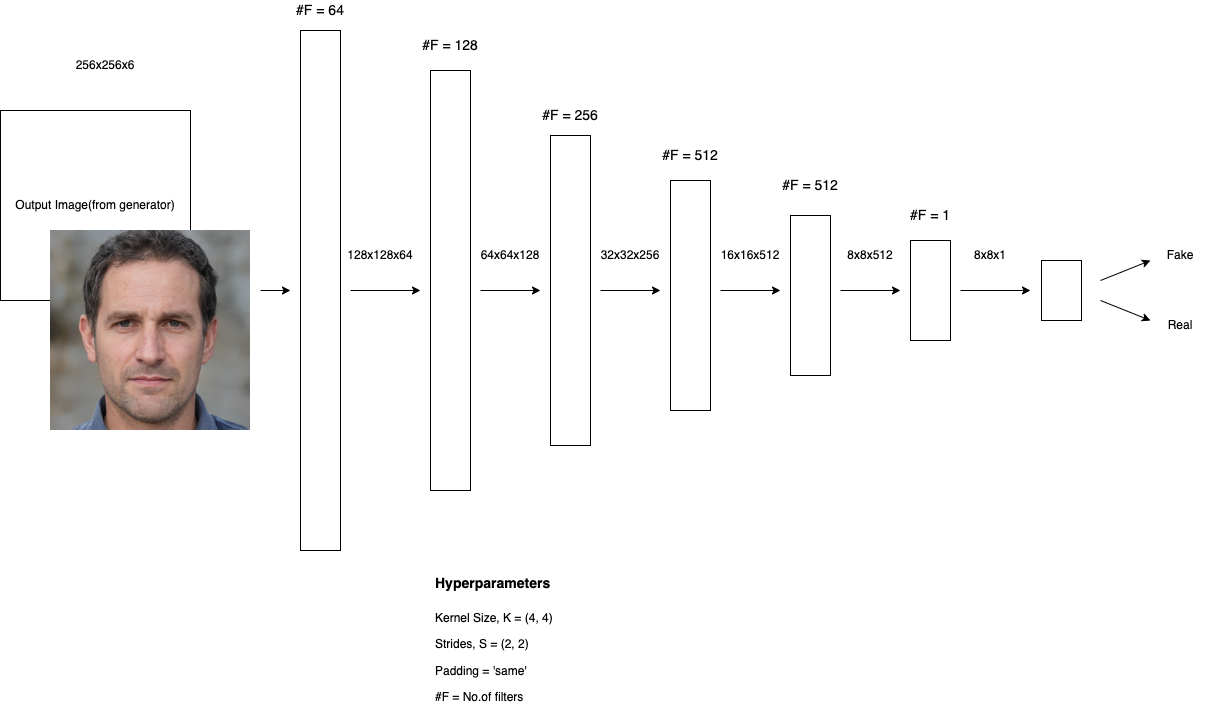
\includegraphics[width=0.95\textwidth]{figures/discriminator.png}
\caption{Architectural Design of Discriminator Model. The input masked picture and the generated unmasked image make up the first input pair, while the input masked image and the actual target image make up the second pair. Before supplying them to the discriminator model, the pictures from a pair are concatenated. The discriminator model attempts to determine if each $NxN$ patch in an image is authentic or fraudulent after the features are down sampled to create $NxN$ patches.}\label{fig3}
\end{figure}

\section{Objective Function}

The Pix2Pix GAN is trained to generate an output $k$ from the observed input $j$ and random noise vector $i$. The loss function can be expressed by:

\begin{equation}
\begin{aligned}
\underset{G}{min}\ \underset{D}{max}\ V(G, D)\ =\ {} & \mathop{\mathbb{E}_{j,k\ \sim\ p_{data}(j, k)} [\log\ D(j, k)]}\ +\ \\
& \mathop{\mathbb{E}_{j\ \sim\ p_{data}(j) , k\ \sim\ p_{data}(k)} [\log\ (1 - D(j, G(j, k)))]}
\label{eq1}
\end{aligned}
\end{equation}

The generator model is simultaneously trained to minimize the generative loss:	

\begin{equation}
L_G\ =\ \mathop{\mathbb{E}_{j\ \sim\ p_{data}(j) , k\ \sim\ p_{data}(k)} [\log\ (1 - D(j, G(j, k)))]}
\label{eq2}
\end{equation}

where the generator strives to reduce the loss function and the discriminator $D$ endeavours to increase it. A greater variety and vividness in produced images are encouraged by the adversarial training process. The generator $G$ is also trained using standard L1 loss in addition to the adversarial loss to represent the pixel-level loss $L_P$ in our model: 

\begin{equation}
L_P = \mathop{\mathbb{E}_{j,k\ \sim\ p_{data}(j,k) , i\ \sim\ p_{data}(i)} [\left\| k - G(j, i) \right\|]}
\label{eq3}
\end{equation}

Therefore, the objective function is defined as:

\begin{equation}
\label{eq4}
L\ =\ w_G\ L_G\ +\ w_P\ L_P\ 
\end{equation}

\section{Experiment and Result}

In our study, we introduced a Pix2Pix model that utilized conditional adversarial networks with the U-net architecture to produce unmasked images from their corresponding masked counterparts. Our evaluation based on Fig 4 indicated that the model generated high-quality unmasked images and received positive feedback from volunteers in a subjective test. However, we observed that the model's performance was limited to the specific masked object used in the data set and struggled to produce high-quality results when faced with other types of masks. To address this issue, our future work will focus on developing a more adaptable model that can handle masks of various shapes and colours.

\begin{figure}[ht]%
\centering
\includegraphics[width=0.95\textwidth]{figures/results0.png}
\caption{. Columns of masked input images, generated unmasked images and actual unmasked image from left.}\label{fig4}
\end{figure}

It can be difficult to assess the quality of a synthesised picture \cite{zhang2016colorful} since conventional measurements like per-pixel mean-squared error don't adequately reflect the properties of the final image. To solve this problem, we ran a poll and collected likeness scores from a group of people to evaluate the precision of our model's unmasked predictions. We gave the participants masked, predicted, and genuine unmasked photographs of various persons from the data set and asked them to assess each image on a scale of 1 to 10 based on its realism because the ultimate aim of our model is to produce aesthetically realistic images. In this study, 46 people in total were recruited for the evaluation procedure.
In order to quantify the evaluation, we define the like index as, like index = $\frac{\sum_{i}^{n}l_i}{n\ast m_r}$ , where $l_i$ is the like measure of the $i^{th}$ individual and $l_i \in [1, 10]$, $n$ is the number of volunteers and is equal to 46 in this study and $m_r$  is the maximum like measure a volunteer can provide. 

Our model's predictions were given a score of 95.5 after applying the like index equation, which showed that the volunteers found the images it produced to be realistic. This subjective evaluation technique gives a more exact and accurate assessment of the visual quality of synthesised pictures, since it considers the subjective experience of the human visual system, which standard metrics fail to capture. 

In summary, our work highlights the relevance of undertaking subjective evaluations to determine the quality of synthesised pictures. We were able to show how well our model produced aesthetically realistic images by using the ratings offered by a group of volunteers. This approach could be further utilized to evaluate other models and facilitate improvements in the field of image synthesis.

\section{Conclusion and Future Work}

In an earlier draught of this paper, we presented a Pix2Pix model for generating the unmasked pictures from the matching masked photos using conditional adversarial networks and the U-net architecture. The predictions shown in Fig 4 lead us to the conclusion that our model does a good job of producing unmasked photos and the subjective test with the various volunteers ensures us that our model has a high like measure. It works well for the masked object utilised in the data set. Despite the encouraging findings, our model struggles to produce high-quality unmasked pictures when various types of masks are used in the input photos. In the future, we will focus on making the model more dynamic that can adjust to masks of varying form and colour.

\section{Acknowledgement}
We would like to extend our gratitude to Prasoon Kottarathil for his gracious donation of the dataset used in this research. Prasoon Kottarathil's Face Mask Lite Dataset, which comprises of masked and equivalent unmasked images produced using StyleGAN \cite{karras2020analyzing}, was crucial to our inquiry since it provided the data we need to conduct our analysis.

\printbibliography

\end{document}